\documentclass[11pt]{article}
\usepackage[utf8]{inputenc}
\usepackage[margin=0.8in]{geometry}
\usepackage{amsfonts, amsmath}
\usepackage{tikz}
\usepackage[nobreak=false]{mdframed}
\usepackage{pgf}
\usepackage{enumitem}
\usepackage{mathtools}
\usepackage{bbold}
\usepackage{graphicx}
\usepackage{url}
\usepackage{enumitem}
\usepackage{amsthm,amssymb}
\usepackage{minted}
\setlength\parindent{0pt}
\newcommand{\solution}{\subsection*{Solution:}}
\DeclareMathOperator*{\argmax}{arg\!max}
\DeclareMathOperator*{\argmin}{arg\!min}
\DeclareMathOperator*{\trace}{trace}
\graphicspath{{./figs/}}

\begin{document}

\title{EE127 Homework 3}
\author{Vighnesh Iyer}
\date{\today}
\maketitle

\subsection*{Exercise 1 (Kantorovich Problem)}

How to move mass $\mu$ to $\nu$ with minimal cost?

\begin{figure}[ht]
\centering
% \includegraphics[width=.45\linewidth]{images/mu_histogram.png}
% \includegraphics[width=.45\linewidth]{images/nu_histogram.png}
\caption{Visualization of $\mu$ histogram on left and $\nu$ histogram on right.}
\label{fig:histogram}
\end{figure}

More rigorously, let $n \in \mathbb{N}$. We define two discrete probability distributions $\mu = (\mu_1, \cdots, \mu_n)$ and $\nu = (\nu_1, \cdots, \nu_n)$ with $\sum_i \mu_i = \sum_i \nu_i = 1$. We define $C = (c_{ij})_{\substack{{1\cdots n} \\ {1\cdots n}}} \in \mathbb{R}_+^{n^2}$ be the cost matrix for transporting one unit of mass from location $i \in [1, \cdots, n]$ to location $j \in [1, \cdots, n]$. The flow matrix $P = (p_{ij})_{\substack{{1 \cdots n} \\ {1 \cdots n}}}$ denotes the quantity of mass to be moved from location $i$ to location $j$. $P$ satisfies the limit conditions:

\[
P \mathbb{1}_n = \mu
\]
\[
P^T \mathbb{1}_n = \nu
\]

\begin{enumerate}

\item What is the total cost of transporting the mass $\mu$ into $\nu$ by following the transportation plan $P$?

\item Write the optimization problem of finding the transportation plan $P$ with minimal cost. What type of optimization problem is it? (LP, QP, $\cdots$?).

\end{enumerate}

The optimal value of the optimization problem you found is a well-defined distance named \emph{Kantorovich} or Wasserstein distance noted $\mathcal{W}(\mu, \nu)$. That distance can be readily applied in the context of document similarity. In particular, while computating the Kantorovich between two documents, we obtain a flow matrix. The point of this question is to show how this matrix can be interpreted. For that, we provide you with a certain prior distance on words (word embeddings) that can be used to compute the transportation cost in the notebook \verb+text-kantorovich.ipynb+.

\begin{enumerate}
\item[3.] Calculate the Wasserstein distance in the notebook using CVX and use visualize the resulting flow matrix $P$ using the provided code. Interpret the results.

\item[4.] Compute the cosine distance between the two given documents. Comment on which distance is more insightful on this precise example and why.\\

\textit{Note: Cosine distance between two documents (or sets of words) is computed as follows. Collect ordered sets of all word counts from both documents. Then compute the cosine of the angle between the two vectors. For example from ``black blue black'' and ``blue blue red'', one would obtain the sets $\{black: 2, blue: 1, red: 0\}$ and $\{black: 0, blue: 2, red: 1\}$. We can then compute the cosine distance between the vectors $[2,1,0]$ and $[0, 2, 1]$.}


\end{enumerate}

We are now interested in computing different barycenters between two discrete vectors $\mu$ and $\nu$ shown in Figure \ref{fig:histogram}. Let us note that the convex combination $t \mu + (1-t) \nu$ has the variational formulation $\operatorname{argmin}_x t(\mu - x)^2 + (1-t) (\nu-x)^2$. Inspired from this fact, we define the variational formulation for convex combinations on the Wasserstein space $\operatorname{argmin}_x t \mathcal{W}(x, \mu) + (1-t) \mathcal{W}(x, \nu)$.

\begin{enumerate}

\item[5.] Write this optimization problem as a LP.

\item[6.] Solve the optimization problem using CVX in the notebook \verb+barycenter.ipynb+. Visualize the Waserstein barycenter for $t \in [0, 0.25, 0.5, 0.75, 1.0]$.

\item[7.] Use your results to comment on the differences between Wasserstein convex combination and euclidean convex combination.
\end{enumerate}

\begin{solution}
\begin{enumerate}
\item
    \begin{align*}
    \sum_{i=1,\dots,n ; j=1,\dots,n} p_{i,j} c_{i,j} = \trace(P \cdot C^T)
    \end{align*}

\item
    \begin{align*}
        \argmin_{\mathbf{P}} &\trace(P \cdot C^T) \\
        \text{Constrained by: }& \\
        P \mathbb{1}_n &= \mu \\
        P^T \mathbb{1}_n &= \nu
    \end{align*}
    This is a LP because the constraints and objective are both linear in the elements of $\mathbf{P}$ which are the variables in this problem. There are $n^2$ variables.

\item To construct the cost matrix:
\begin{minted}[breaklines,tabsize=2]{python}
C = [[distance(document_1[w_1],document_2[w_2]) for w_2 in range(len(document_2))] for w_1 in range(len(document_1))]
\end{minted}
Then I constructed $A$ which was the equality constraint matrix as such:
\begin{minted}[breaklines,tabsize=2]{python}
flatten = lambda l: [item for sublist in l for item in sublist]
A_top_1 = np.array(flatten([[1]*l, [0]*l*(l-1)]))
A_top = np.array([np.roll(A_top_1, n*l) for n in range(l)])
A_bot_1_bit = flatten([[1], [0]*(l-1)])
A_bot = np.array([np.tile(np.roll(A_bot_1_bit, n), l) for n in range(l)])
A = np.vstack((A_top, A_bot))
print(A)
\end{minted}
\begin{minted}{text}
[[1 1 1 1 0 0 0 0 0 0 0 0 0 0 0 0]
 [0 0 0 0 1 1 1 1 0 0 0 0 0 0 0 0]
 [0 0 0 0 0 0 0 0 1 1 1 1 0 0 0 0]
 [0 0 0 0 0 0 0 0 0 0 0 0 1 1 1 1]
 [1 0 0 0 1 0 0 0 1 0 0 0 1 0 0 0]
 [0 1 0 0 0 1 0 0 0 1 0 0 0 1 0 0]
 [0 0 1 0 0 0 1 0 0 0 1 0 0 0 1 0]
 [0 0 0 1 0 0 0 1 0 0 0 1 0 0 0 1]]
\end{minted}
Then construct $b$ which was the equality constraint vector:
\begin{minted}{python}
b = np.hstack((mu,nu))
print(b)
[0.25 0.25 0.25 0.25 0.25 0.25 0.25 0.25]
\end{minted}
Now solve:
\begin{minted}{python}
x = opt.linprog(c, A_eq=A, b_eq=b)
P = np.reshape(x.x, (l,l))
emd = x.fun
print("EMD: " + str(emd))
print(x.x)
EMD: 2.8658661246299744
x: array([0., 0., 0.25, 0., 0., 0., 0., 0.25, 0., 0.25, 0., 0., 0.25, 0., 0., 0.])
\end{minted}
\begin{figure}[H]
    \centerline{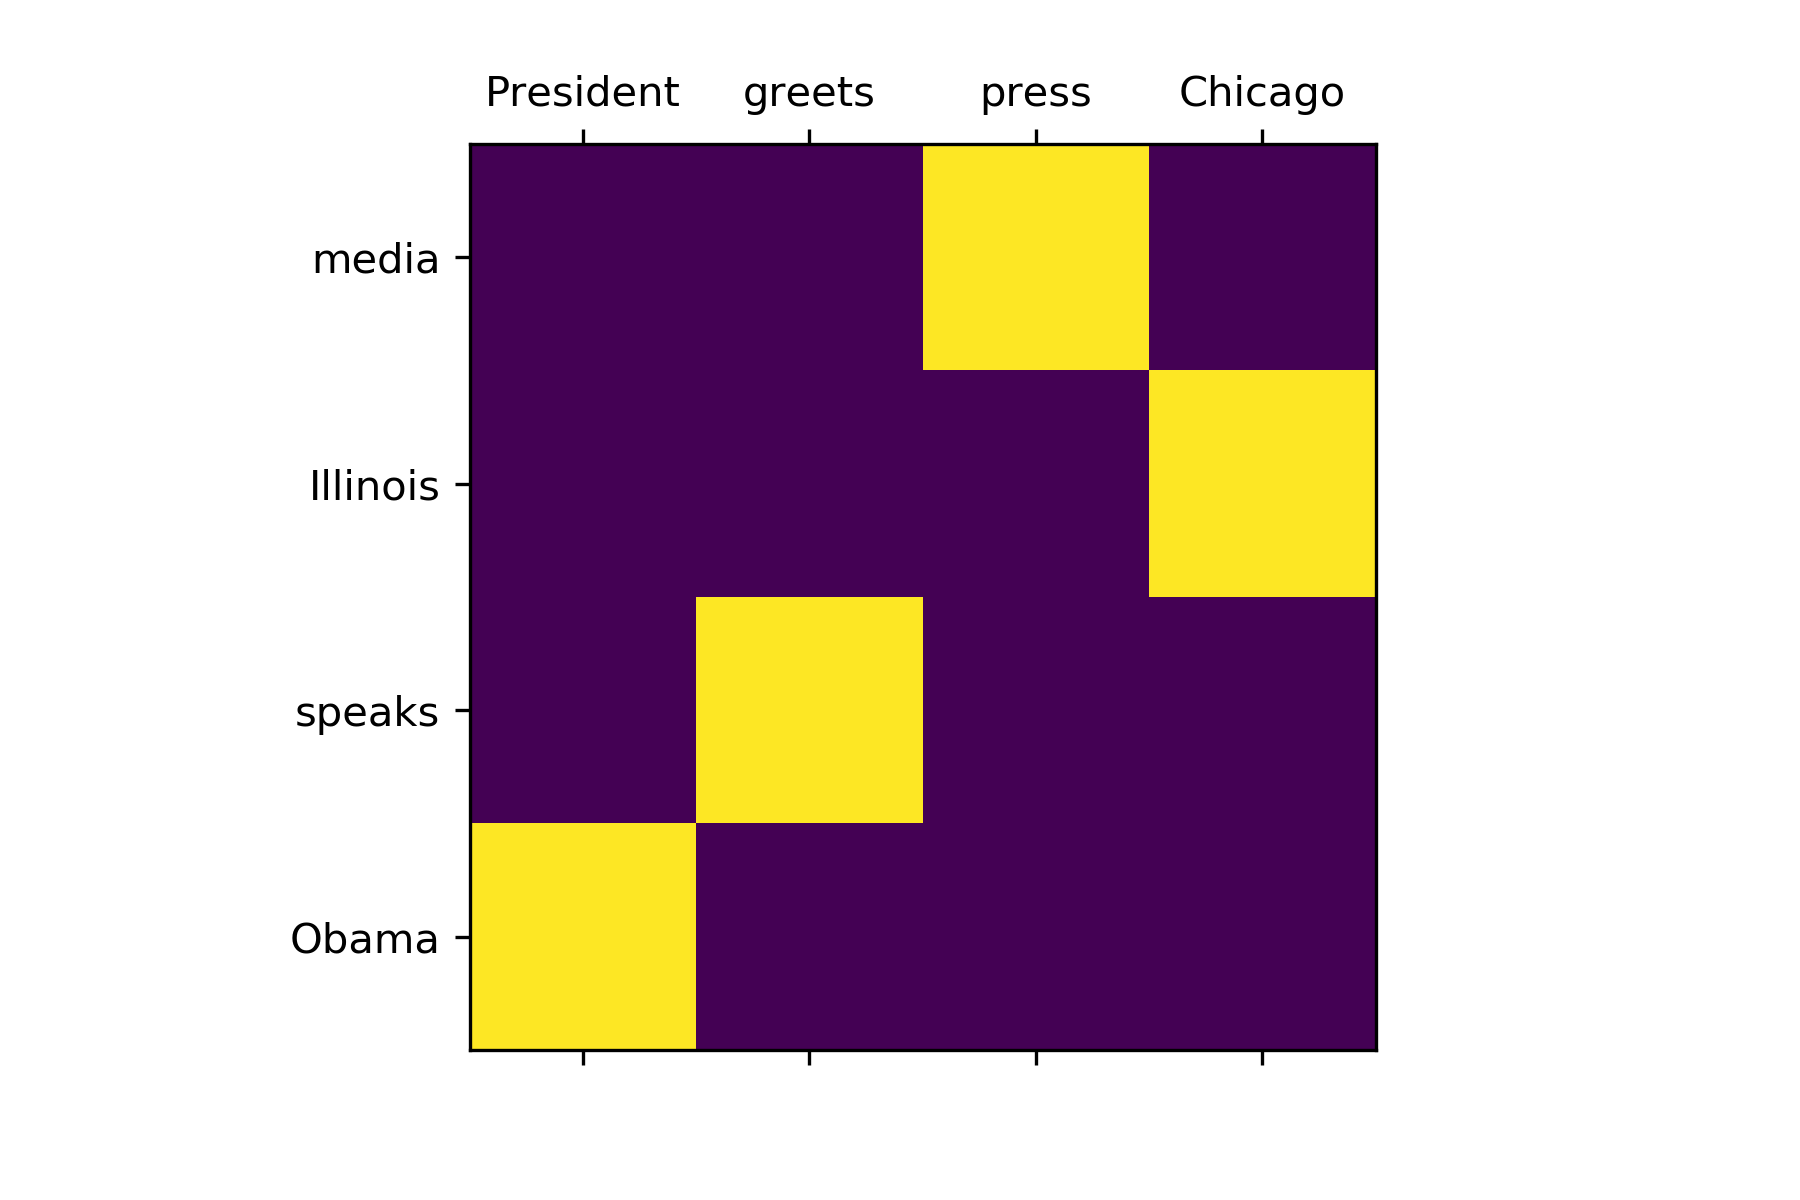
\includegraphics[width=0.4\textwidth]{problem1_kantorovich_plan.png}}
\end{figure}

\item The cosine distance is just 0 (due to orthogonal word frequency vectors) because the two documents share no words in common.

The Kantorovich distance is more insightful in this example because it relates the 'logical' (from the cost matrix) difference between two words rather than the literal (character by character) difference.

\item We can write the optimization problem as an LP:
\begin{align*}
    &\argmin_{x} t \mathcal{W}(x,\mu) + (1-t)\mathcal{W}(x,\nu) \\
    &\argmin_{x} t \min_{\mathbf{P'}} \trace(P' \cdot C^T) + (1-t) \min_{\mathbf{P''}} \trace(P'' \cdot C^T) \\
    &\min_{\mathbf{P'},\mathbf{P''}} t \trace(P' \cdot C^T) + (1-t) \trace(P'' \cdot C^T)
\end{align*}
This objective function is now linear in the elements of the $\mathbf{P'},\mathbf{P''}$ matrices. The constraints are linear in $x \in \mathbb{R}^n$ and $\mathbf{P'}, \mathbf{P''}$:
\begin{align*}
    P' \mathbb{1}_n - x &= 0 \\
    P'' \mathbb{1}_n - x &= 0 \\
    P'^T \mathbb{1}_n &= \mu \\
    P''^T \mathbb{1}_n &= \nu
\end{align*}

\item I constructed the $A$, $b$, and $c$ matrices "manually". Here are the distributions for $\mu$ and $\nu$.

\begin{figure}[H]
    \centerline{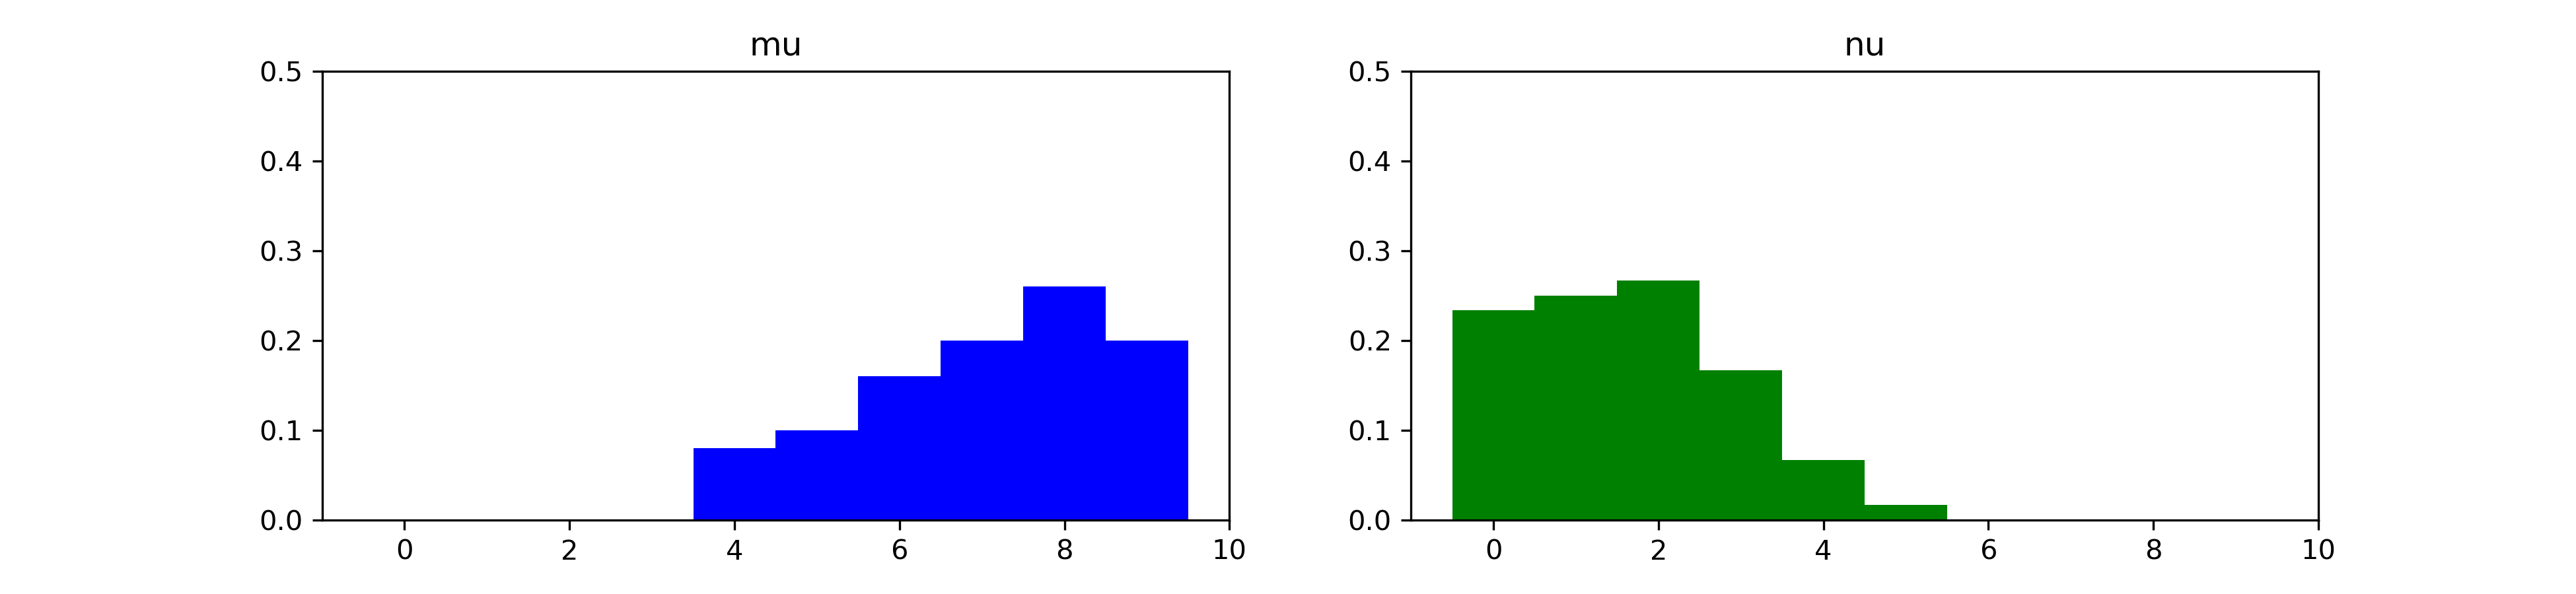
\includegraphics[width=0.7\textwidth]{problem1_mu_nu.png}}
\end{figure}

Here is a comparison between the Euclidean and Wasserstein barycenters.
\begin{figure}[H]
    \centerline{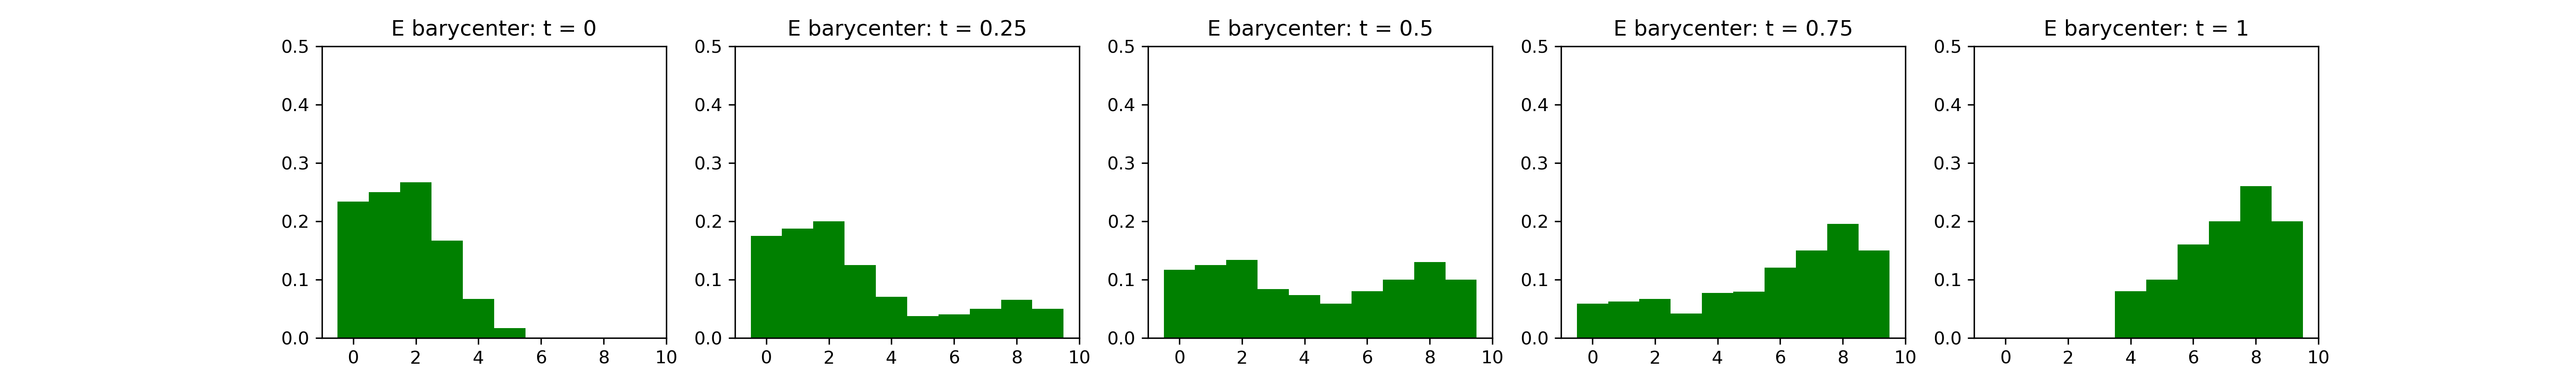
\includegraphics[width=\textwidth]{problem1_e_barycenter.png}}
    \centerline{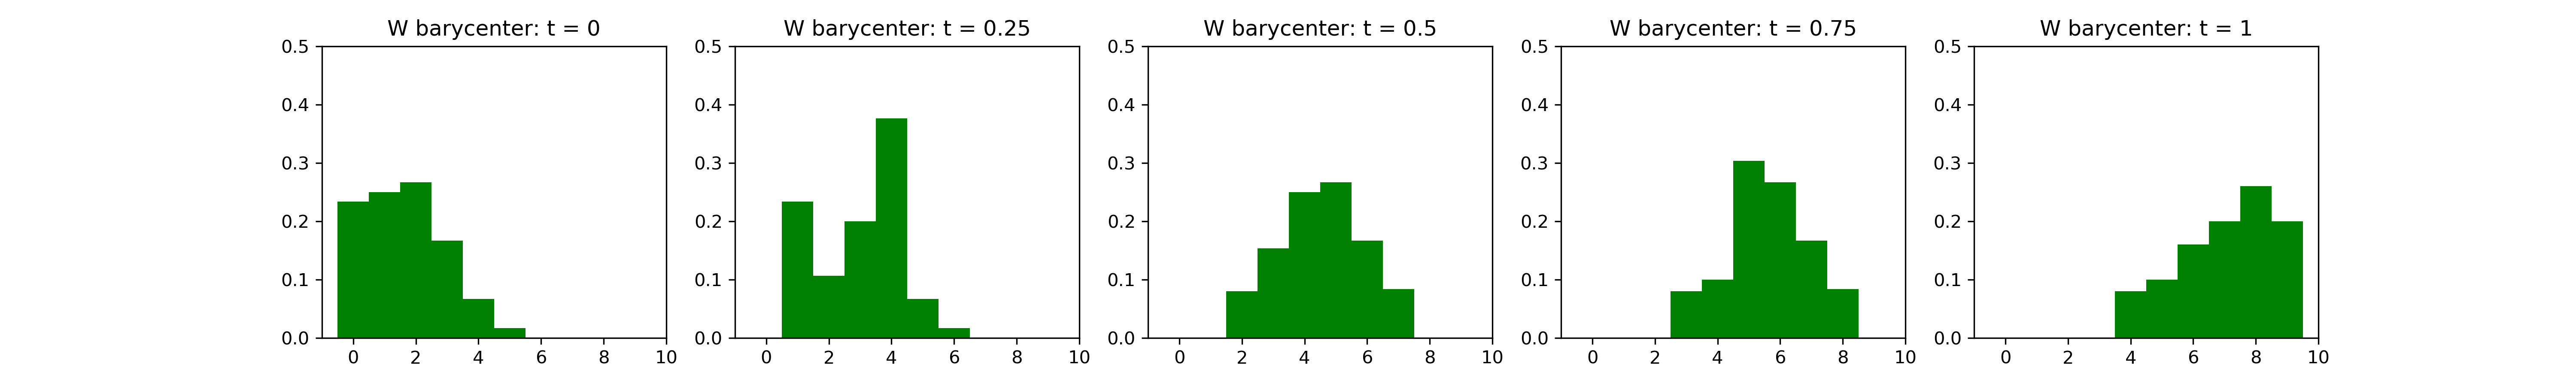
\includegraphics[width=\textwidth]{problem1_w_barycenter.png}}
\end{figure}

\item The Euclidean barycenter is just an averaging of the two distributions (in the $t = 0.5$ case), but the W barycenter intelligently moves the mass of both distributions by the minimal amount to satisfy the constraints, which gives a much better 'center of gravity' representation. The W barycenter converges to the Euclidean one for $t = 0,1$.
\end{enumerate}
\end{solution}

\newpage
\subsection*{Exercise 2 (Fast CV for Least-Squares)}

In this exercise, we consider a regularized least-squares problem:
\begin{equation}\label{eq:rls}
w_\lambda :=\arg\min_w \: \|y-Xw\|_2^2 + \lambda \|w\|_2^2,
\end{equation}
with $X \in \mathbb{R}^{n \times p}$ the data matrix (with one data point per row), $y \in \mathbb{R}^n$ is the response vector, and $\lambda>0$ a ``ridge'' regularization parameter. Solving the above problem leads to a prediction model: for a new data point $x \in \mathbb{R}^{p}$, $\hat{y}(x) = w_\lambda^\top x$.

We would like to choose this regularization parameter based on the notion of ``leave-one-out''  (LOO) cross-validation, whereby for a given candidate value of $\lambda>0$, we estimate the resulting prediction error, averaged across all the models given by the above, when leaving out one data point. Precisely, we set, for $i=1,\ldots,n$
\[
w^{(i)}_\lambda := \arg\min_w \: \|y_{\backslash i}-X_{\backslash i}w\|_2^2 + \lambda \|w\|_2^2,
\]
with $X_{\backslash i}$ (resp.\ $y_{\backslash i}$) is equal to $X$ (resp. $y$), with the $i$-th row (resp.\ element) removed, and evaluate the prediction error on the point we just left out, with $\hat{y}(x_i) = x_i^\top w^{(i)}_\lambda$.

Obviously, we can compute the LOO error by simply solving $n$ problems of the form~(\ref{eq:rls}), with the appropriate data. In this exercise we investigate a faster method, which is based on solving the above full problem \emph{once}, then performing cheap updates to get the LOO error.

\begin{enumerate}
    \item Show that the solution to the full problem is of the form
    \[
    w_\lambda = (X^\top X+\lambda I)^{-1}X^\top y
    \]
    \item Prove a (simple) version of the Sherman-Morrison-Woodbury identity. Given $M=A+uv^\top$ (with $A$ symmetric/invertible, $A+uv^\top$ also invertible) show that
    \begin{align}
        M^{-1} = A^{-1}-\frac{1}{1+v^\top A^{-1} u} (A^{-1} u)(A^{-1} v)^\top
    \end{align}
    Namely, it is sufficient to just show that $MM^{-1}=I$ (since showing $M^{-1}M=I$ is similar).
    \item Argue both $X_{\backslash i}^\top X_{\backslash i}$ and $X_{\backslash i}^\top y_{\backslash i}$ can be written as rank-one modifications of $X^\top X$ and $X^\top y$ and show that,
    \[
    w^{(i)}_\lambda = w - \frac{\Sigma^{-1} x_i e_i}{1-h_i}
    \]
    where we define $\Sigma = X^\top X+\lambda I$, $h_i = x_i^\top \Sigma^{-1} x_i$, and $e_i = y_i - x_i^\top w_{\lambda}$ for convenience.
    {\em Hint: use the Sherman-Morrison-Woodbury identity.}

    \item Compute (and simplify) the LOO prediction error $\frac{1}{n} \sum_{i=1}^{n} (y_i-(w^{(i)}_{\lambda})^\top x_i)^2$ into an expression consisting of $e_i, h_i$.

    \item What is the complexity of the method for computing the LOO prediction error investigated in this problem relative the naive method where we compute all $w_{\lambda}^{(i)}$ without reusing computations? Highlight the leading dependencies in terms of $n, p$ for both methods in big-$O$ notation.
\end{enumerate}

\begin{solution}
% Your solution here
\end{solution}


\newpage
\subsection*{Exercise 3 (Least norm estimation on traffic flow networks)}

In this problem, we want to estimate the traffic given the road network as well as the historical average of flows on each road segment. We call $q_i$ the flow of vehicles on each road segment $i\in I$. At each intersection, the sum of all incoming flows must be equal to the sum of all outgoing flows. We construct the matrix $A \in \mathbb{R}^{J\times I}$ such that the element on the $j$th line and $i$th column is
\begin{itemize}
\item $0$ if link $i$ does not arrive or leave intersection $j$;
\item $1$ if link $i$ arrives at intersection $j$;
\item $-1$ if link $i$ leaves intersection $j$.
\end{itemize}

\begin{enumerate}
\item Write down the linear equation that corresponds to the conservation of vehicles at each intersection $j\in J$.

\item The goal is to estimate the traffic flow on each of the road segment. The flow estimates should satisfy the conservation of vehicles exactly at each intersection. Among the solutions that satisfy this constraint, we are searching for the estimate that is the closest to the historical average, $\overline{q}$, in the $l_2$-norm sense. The vector $\overline{q}$ has size $I$ and the $i$-th element represent the average for the road segment $i$. Pose the optimization problem.

\item Find a closed form solution to this problem. Detail your answer (do not only give a formula but explain where it comes from).

\begin{figure}[!ht]
\centering
% \includegraphics[width=.6\linewidth]{images/TrafficFlow.pdf}
\caption{Example of traffic estimation problem. The intersections are labeled $a$ to $h$. The road segments are labeled 1 to 22. The arrows indicate the direction of traffic.}
\label{fig:flows}
\end{figure}
\item Formulate the problem for the small example of Figure~\ref{fig:flows} and solve it using the historical average given in Table~\ref{tab:lineqs:historical_flows}. What is the flow that you estimate on road segments 1, 3, 6, 15 and 22?

\item Now, assume that besides the historical averages, you are also given some flow measurements on some of the road segments of the network. You assume that these flow measurements are correct and want your estimate of the flow to match these measurements perfectly (besides matching the conservation of vehicles of course). The right column of
Table~\ref{tab:lineqs:historical_flows}
lists the road segments for which we have such flow measurements. Do you estimate a different flow on some of the links? Give the difference in flow you estimate for road segments 1,3, 6, 15 and 22. Also check that you estimate gives you the measured flow on the road segments for which you have measured the flow. {\em Hint:} Your solution will comment on the feasibility of solving such a problem.

\end{enumerate}

\begin{solution}
\begin{enumerate}
\item The sum across each row in the matrix $A$ must be 0.
\begin{align*}
    A \mathbb{1}_I = \mathbb{0}_J
\end{align*}

\item
\begin{align*}
    \min_q &\|q - \overline{q}\|_2^2 \\
    \text{subject to } & A q = \mathbb{0}_J
\end{align*}

\item This is a constrained least-squares problem.
\begin{align*}
    \text{Let } q = N z \\
    \text{where } N &\text{ is a matrix formed by a columnar basis for the nullspace of } A \\
    \text{and where } z& \text{ is a free variable} \\
    \min_z &\|Nz - \overline{q}\|_2^2
\end{align*}
        This is in standard least squares configuration with $N$ having full column rank (because I > J and $dim(N) = $ (I, I-J)), so the solution:
\begin{align*}
    z^* &= (N N^T)^{-1} N^T \overline{q} \\
    q^* &= N z^*
\end{align*}

\item I used the following Python:
\begin{minted}{python}
I = 22
J = 8
J_lookup = {
    0: [(1, 1), (5, 1), (6, -1), (10, 1)],
    1: [(6, 1), (7, -1), (2, -1), (11, -1)],
    2: [(3, 1), (7, 1), (8, -1), (12, 1)],
    3: [(4, -1), (8, 1), (9, -1), (13, -1)],
    4: [(10, -1), (14, -1), (19, 1), (15, 1)],
    5: [(11, 1), (15, -1), (16, 1), (20, -1)],
    6: [(12, -1), (16, -1), (17, 1), (21, 1)],
    7: [(13, 1), (17, -1), (18, 1), (22, -1)]
}
A = np.zeros((J, I))
for j in range(J):
    for (i, val) in J_lookup[j]:
        A[j,i-1] = val
print(np.shape(A))
q = [2047.6, 2046.0, 2002.6, 2036.9, 2013.5,
    2021.1, 2027.4, 2047.1, 2020.9, 2049.2,
    2015.1, 2035.1, 2033.3, 2027.0, 2034.9,
    2033.3, 2008.9, 2006.4, 2050.0, 2008.6,
    2001.6, 2028.1]
N = (scipy.linalg.null_space(A))
print(np.shape(N))
\end{minted}
\begin{minted}{text}
(8, 22)
(22, 14)
\end{minted}
\begin{minted}{python}
z_star = np.dot(np.dot(np.linalg.inv(np.dot(N.T, N)), N.T), q)
print(z_star)
q_star = np.dot(N, z_star)
print(q_star)
print(np.linalg.norm(np.dot(A, q_star)))
print(np.linalg.norm(q - q_star))
\end{minted}
\begin{minted}{text}
[1208.69323821 1767.51345581 -860.89380776 1522.45159784 -875.97214974
 3221.36721742 3194.08194262  551.24629765 3234.46993025  -90.66538795
  855.63278258 4362.14916004 1130.1045423  4125.16538795]
[1137.50891932 1390.98449431 1371.28133641 1131.5415509  1103.40891932
 3586.20658637  741.06583072 3583.77711269 1115.5415509  1345.28874773
 1454.15626134 1471.42994555 1336.69401089 2233.17982841 1734.64840455
 2195.02037618 1732.49893087 2215.15245999 1843.82017159 1914.52823296
 1933.95139086 1819.34754001]
2.008109928812666e-12
3546.9021413285463
\end{minted}

To check my solution, I used a generic optimizer:
\begin{minted}[breaklines]{python}
res = scipy.optimize.minimize(lambda x: np.linalg.norm(x - q)**2, method='SLSQP', x0 = q, constraints = {
    'type': 'eq',
    'fun': lambda x: np.dot(A, x)
})
print(np.linalg.norm(np.dot(A, res.x)))
print(np.linalg.norm(q - res.x))
print(np.linalg.norm(res.x - q_star))
\end{minted}
\begin{minted}{text}
1.8331451766013172e-12
3546.902148694427
0.22858721834675316
\end{minted}

On the specific segments:
\begin{minted}[breaklines]{python}
print(q_star[0], q_star[2], q_star[5], q_star[14], q_star[21])
1137.508919320243 1371.2813364131339 3586.2065863718854 1734.6484045537036 1819.3475400098991
\end{minted}

\item To find the new $q^*$ with the fixed values, I just added another constraint to the generic optimizer.
\begin{minted}{python}
m = [2028, 2008, 2035, 0, 2019, 0, 0, 0, 2044, 0, 0, 0, 0, 2043, 0, 0, 0, 0, 2030, 2025, 0, 2045]
A_m = np.diag([1, 1, 1, 0, 1, 0, 0, 0, 1, 0, 0, 0, 0, 1, 0, 0, 0, 0, 1, 1, 0, 1])
res_m = scipy.optimize.minimize(lambda x: np.linalg.norm(x - q)**2, method='SLSQP', x0 = q, constraints = [{
    'type': 'eq',
    'fun': lambda x: np.dot(A, x)
}, {
    'type': 'eq',
    'fun': lambda x: np.linalg.norm(np.dot(A_m, x) - m)
}])
print(res_m.x)
print(res.x)
\end{minted}
\begin{minted}{text}
[2027.99999879 2008.00000043 2034.9999992  1224.47183591 2018.99999868
 4887.95746125 1342.44541946 4513.36550797 2043.99999951  840.95746462
 1537.51204219 1135.92009013 1244.89367338 2043.00000073  853.95746615
 1341.44542435 1230.2744971  2030.38082348 2029.9999992  2025.00000039
 1247.09101737 2044.99999975]
[1137.54054666 1391.07730127 1371.3558991  1131.59313753 1103.410788
 3586.27483531  741.04331072 3583.86260257 1115.54879952 1345.32350064
 1454.15422332 1471.46339275 1336.72066553 2233.19578875 1734.66255519
 2195.06862522 1732.51280106 2215.21249473 1843.85673421 1914.56029335
 1934.01921691 1819.4203592 ]
\end{minted}

Some of the links have very different values.
\begin{minted}[breaklines]{python}
print(res.x[0] - res_m.x[0], res.x[2] - res_m.x[2], res.x[5] - res_m.x[5], res.x[14] - res_m.x[14], res.x[21] - res_m.x[21])
-890.4594521237909 -663.6441001042463 -1301.6826259366453 880.7050890380153 -225.57964055374282
\end{minted}

This problem seems feasible in this case, since these are just new linear constraints on a LS problem and we have enough free variables to account for the flow differences the new constants cause and still maintain the conservation constraint.

This could become an issue when you don't have enough free variables to handle new fixed equality constraints.
\end{enumerate}
\end{solution}

\newpage
\subsection*{Exercise 4 (A Portfolio Design Problem)}

The returns on $n = 4$ assets are described by a Gaussian (normal) random vector $r \in \mathbb{R}^n$ , having the following expected value $\hat{r}$ and covariance matrix $\Sigma$:
\[
\hat{r} =
\begin{bmatrix}
    0.12  \\
    0.10  \\
    0.07 \\
    0.03

\end{bmatrix}, \; \Sigma =
\begin{bmatrix}
    0.0064 & 0.0008 & -0.0011  & 0 \\
    0.0008 & 0.0025 & 0  & 0 \\
    -0.0011 & 0 & 0.0004  & 0 \\
    0 & 0 & 0  & 0

\end{bmatrix}
.
\]


The last (fourth) asset corresponds to a risk-free investment. An investor
wants to design a portfolio mix with weights $x \in \mathbb{R}^n$ (each weight $x_i$
is non-negative, and the sum of the weights is one) so as to obtain the best possible expected return $\hat{r}^Tx$, while guaranteeing that: \\

(i) No single asset weights more than $40\%$ \\
(ii) The risk-free assets should not weight more than $20\%$ \\
(iii) No asset should weight less than $5\%$ \\
(iv) The probability of experiencing a return lower than $q = -3\%$ should be no larger than $\epsilon = 10^{-4}$
\begin{enumerate}
\item
What is the maximal achievable expected return, under the above constraints? \\

\textbf{Hint}: Constraint (iv) is known as a "chance constraint."
\[
a^Tx \sim N(\hat{a}, \Sigma) \implies a^Tx - b \sim N(\hat{a}x - b, x^Tx\Sigma x).
\]
We then have:
\[\Pr(a^Tx \leq b) \geq \eta \iff b - \hat{a}^Tx \geq \Phi^{-1}(\eta)||\Sigma^{1/2}x||_2
\]

\item Solve the problem for a large number of values of $\epsilon$ between $10^{-4}$ and $10^{-1}$, and plot the optimal values of $\hat{r}^Tx$ versus $\epsilon$. Also make an area plot of the optimal portfolios $x$ versus $\epsilon$.

\item \textit{Monte Carlo simulation.} Let $x$ be the optimal portfolio found in part 1, with $\epsilon=10^{-4}$. This portfolio maximizes the expected return, subject to the probability of a loss being no more than 3 $\%$. Generate 1000 samples of $r$, and plot a histogram of the returns. Find the empirical mean of the return samples, and calculate the percentage of samples for which a loss occurs.

\end{enumerate}

\begin{solution}
\begin{enumerate}
  \item We can solve this directly using CVXPY:
    \begin{minted}{python}
import cvxpy as cp
from cvxpy.atoms.norm import norm
from cvxpy.atoms.affine.sum import sum

x = cp.Variable(4)
objective = cp.Maximize(r_hat @ x)
constraints = [x >= 0.05,
               x <= 0.4,
               x[3] >= 0.2,
               norm(sigma_sqrt @ x) <= (1/epsilon)*(-0.03 - (r_hat @ x)),
               sum(x) == 1]
prob = cp.Problem(objective, constraints)

result = prob.solve()
print(result)
print(x.value)
0.09249999999756837
[0.4  0.35 0.05 0.2 ]
    \end{minted}
    The expected max return is 9.25\%

  \item I swept $\epsilon$ from 10e-5 to 10e-1, since I didn't observe any interesting behavior below $\epsilon$ = 10e-3.
    \begin{figure}[H]
      \centerline{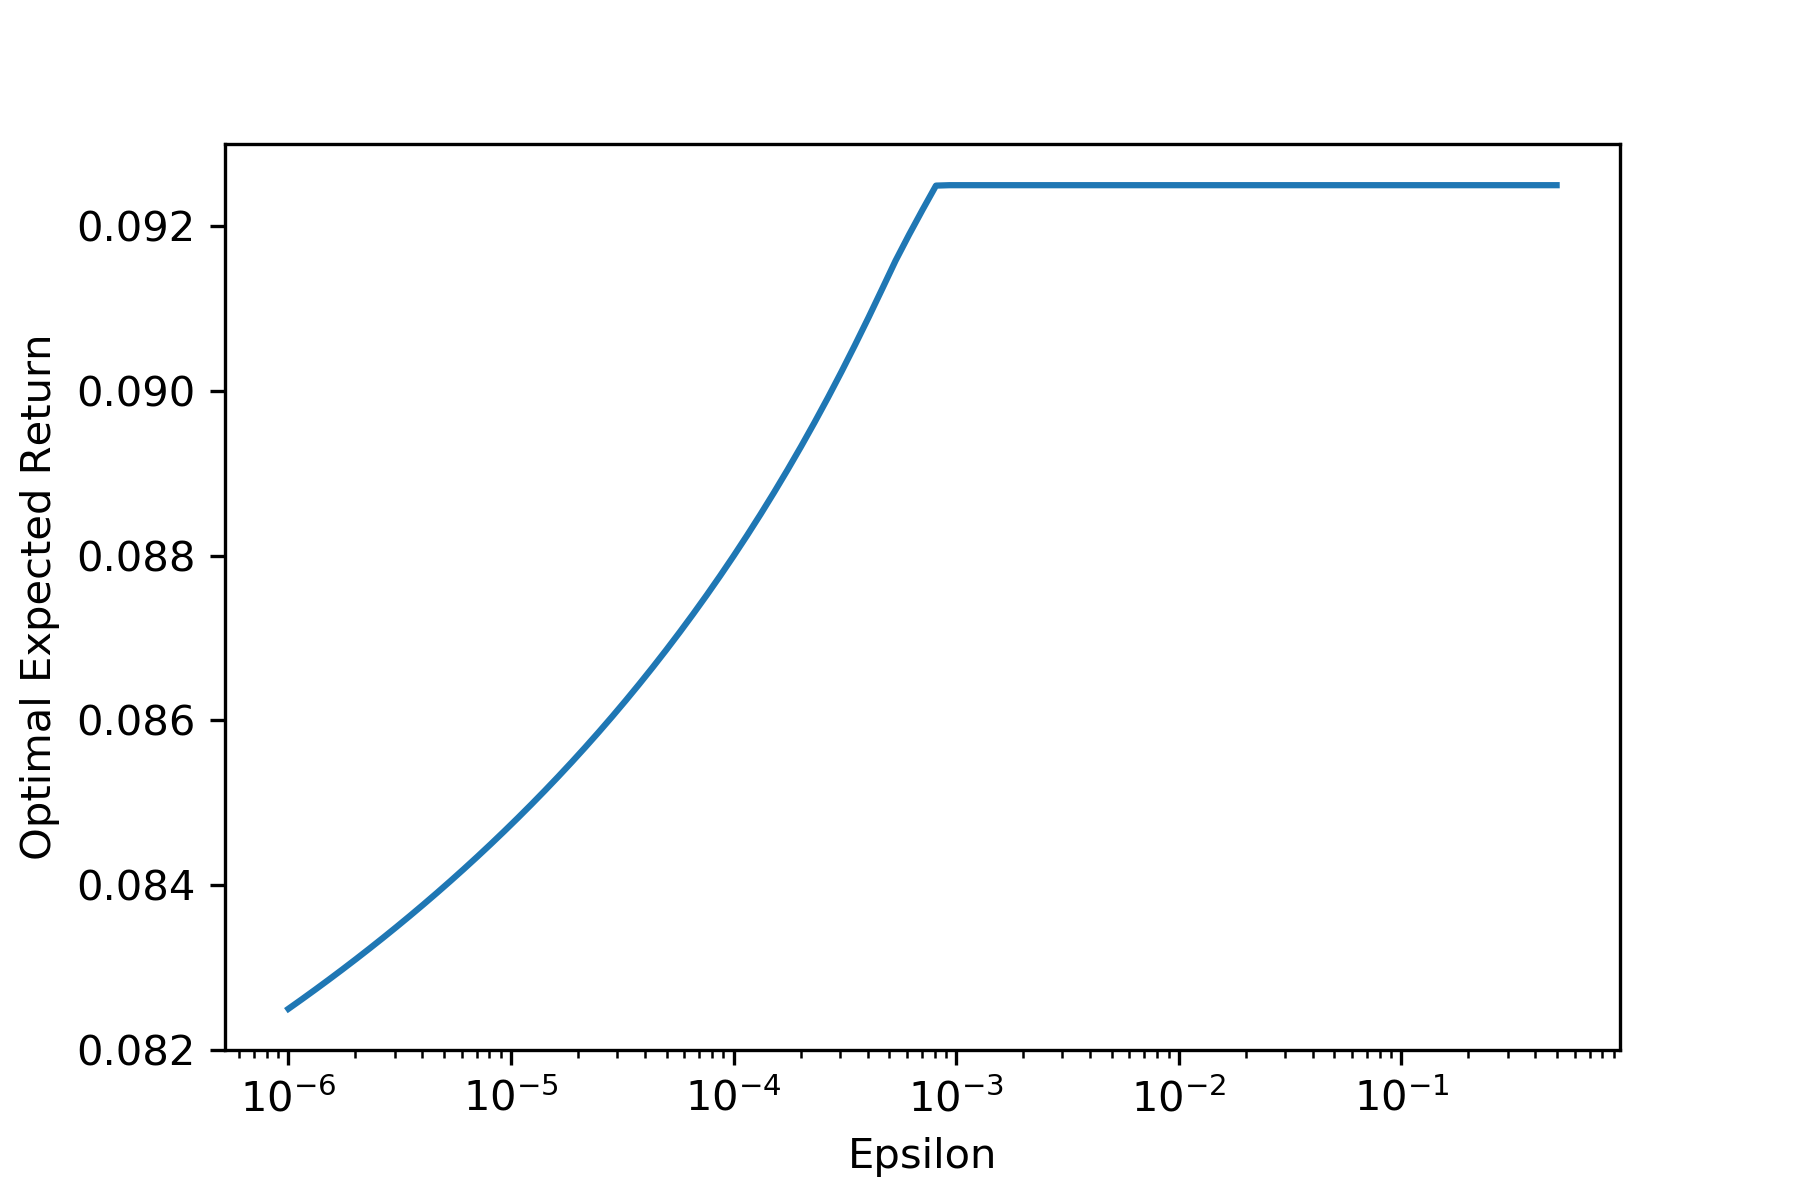
\includegraphics[width=0.5\textwidth]{problem4_sweep_epsilon.png}}
      \centerline{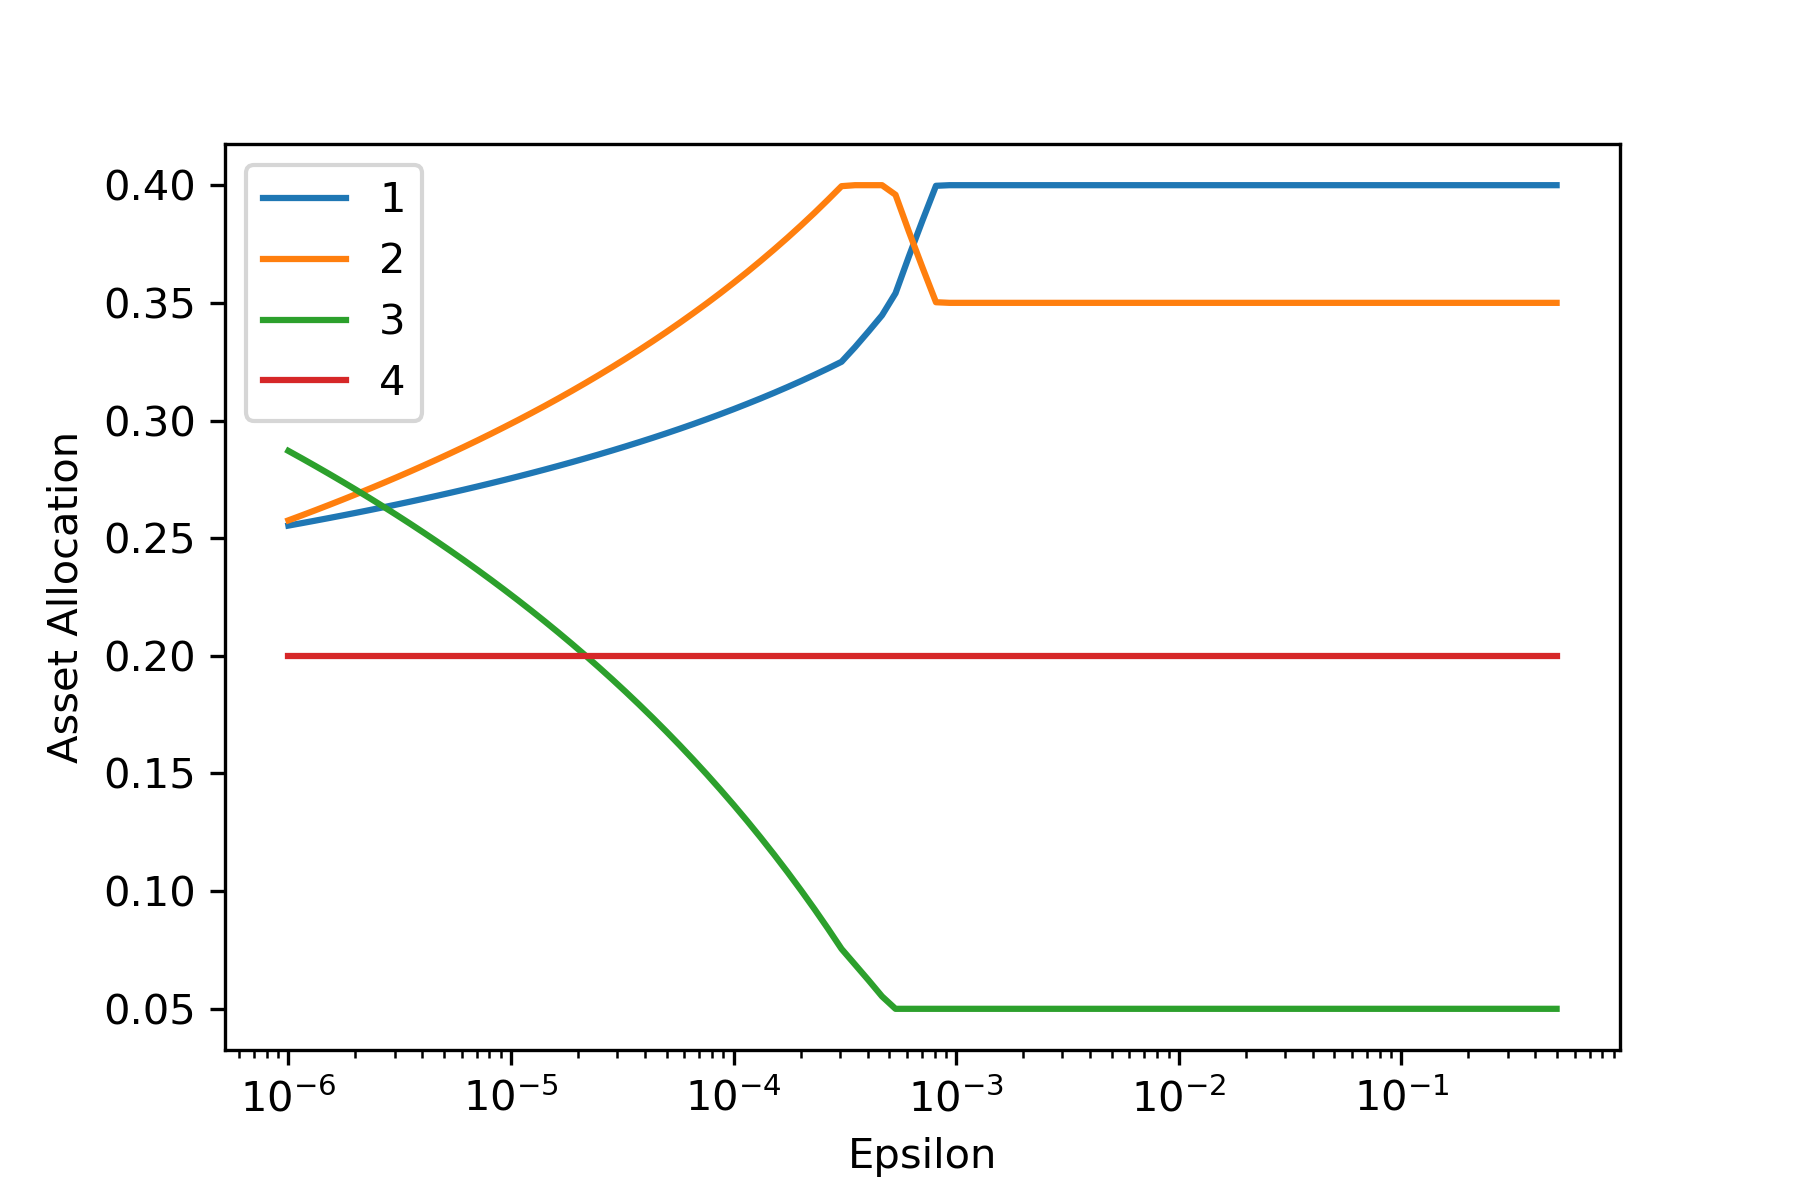
\includegraphics[width=0.5\textwidth]{problem4_area_plot.png}}
    \end{figure}

  \item Histogram from 1000 samples of $r$.
    \begin{figure}[H]
      \centerline{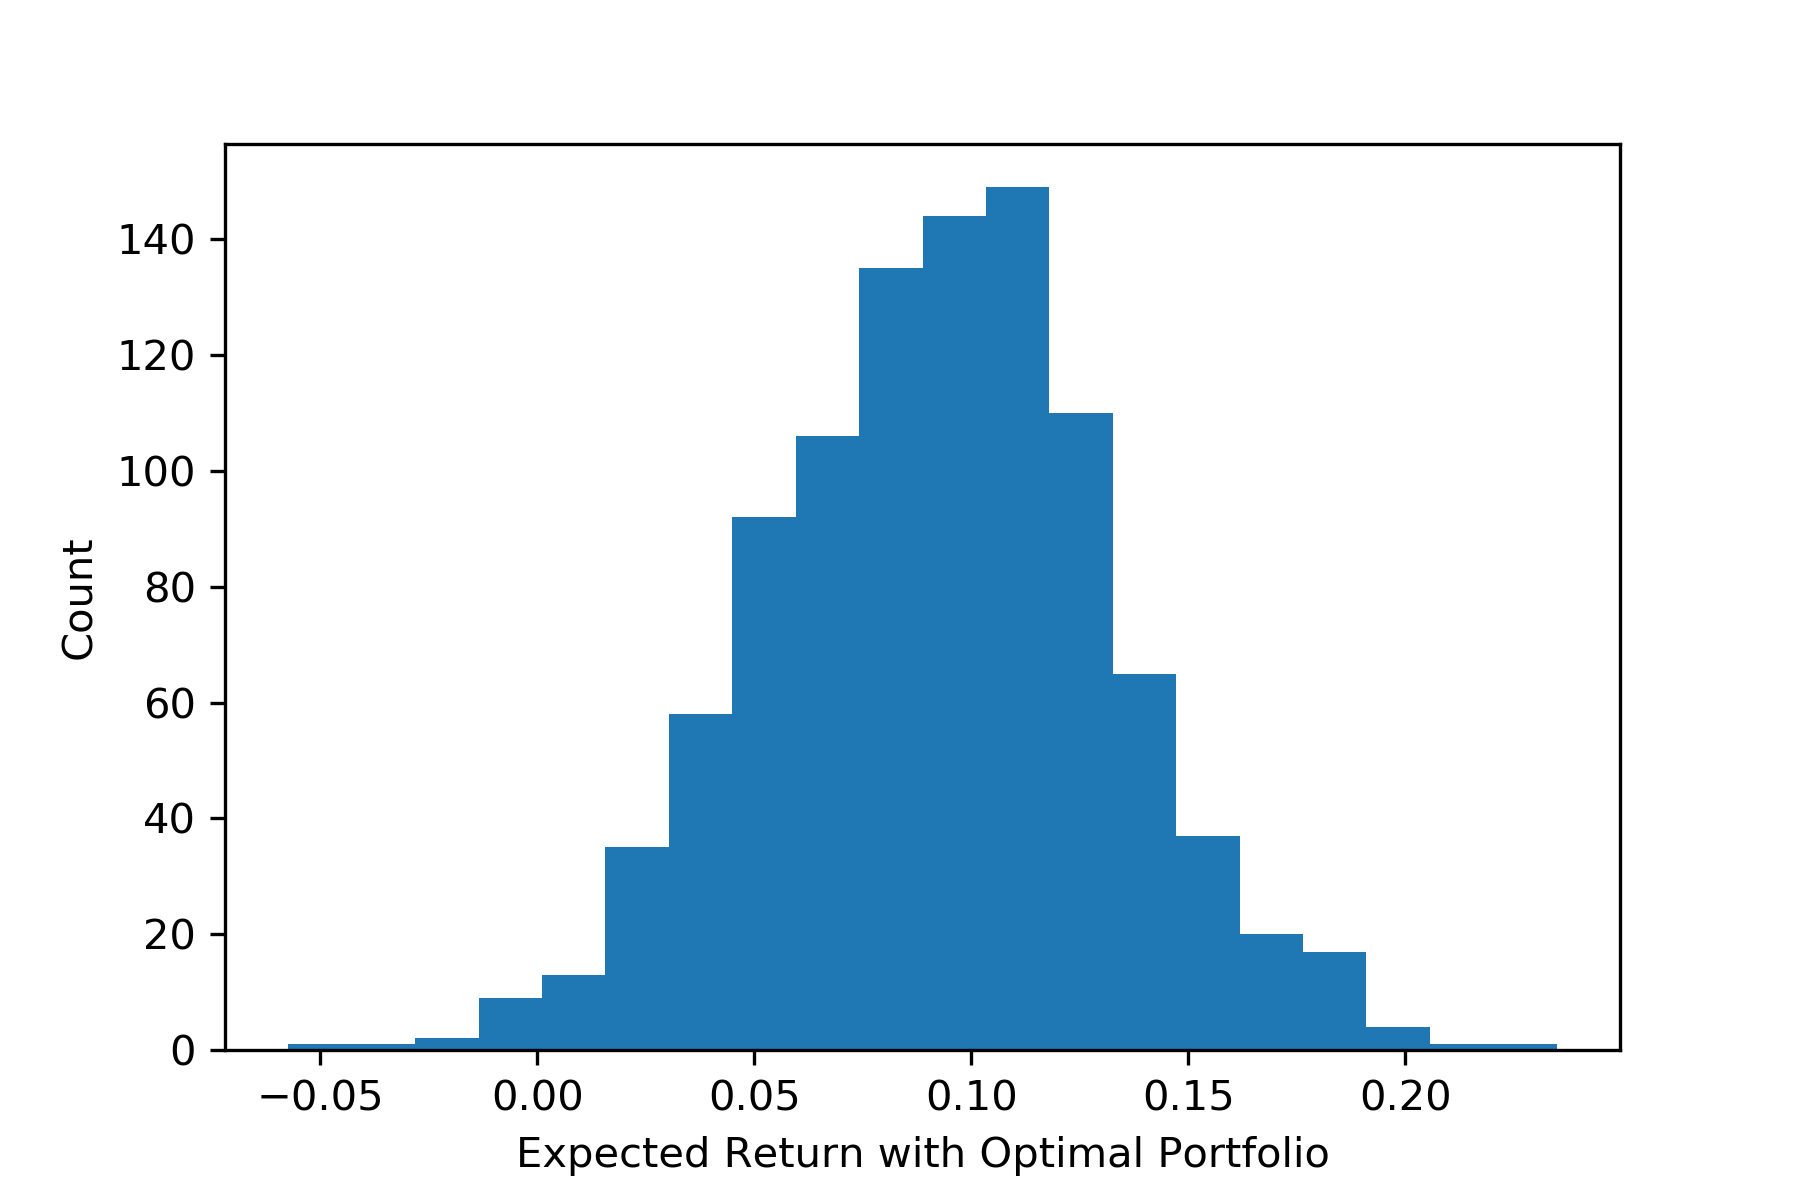
\includegraphics[width=0.5\textwidth]{problem4_monte_carlo.png}}
    \end{figure}

    The mean return is 0.0921 and 1.3\% of the samples had a loss. 0.2\% of the samples had a loss greater than or equal to 3\%, which is close to the original constraint.
\end{enumerate}
\end{solution}

\newpage
\subsection*{Exercise 5 (A slalom problem)}

A two-dimensional skier must slalom down a slope, by going through $n$ parallel gates of known position $(x_i,y_i)$, and of width $c_i$, $i=1,\ldots,n$. The initial position $(x_0,y_0)$ is given, as well as the final one, $(x_{n+1},y_{n+1})$. Here, the $x$-axis represents the direction down the slope, from left to right, see Figure~\ref{fig:slalom_pic.pdf}. \\


\begin{figure}[h]
\begin{center}
% \includegraphics{slalom_pic.pdf}
%[width=.45\textwidth,height=.25\textheight,angle=0]
\end{center}
\caption{\label{fig:slalom_pic.pdf}  Slalom problem with $n=5$ obstacles. ``Uphill'' (resp.\ ``downhill'') is on the left (resp.\ right) side. The middle path is dashed, initial and final positions are not shown.}
\end{figure}

\begin{table}[h]
\begin{center}
\[
\begin{array}{c|ccc}
i & x_i & y_i & c_i \\\hline
0 & 0 & 4 & N/A \\
1 & 4 & 5 & 3 \\
2 & 8 & 4 & 2 \\
3 & 12 & 6 & 2 \\
4 & 16 & 5 & 1 \\
5 & 20 & 7 & 2 \\
6 & 24 & 4 & N/A
\end{array}
\]
\end{center}
\caption{Problem data for Exercise~\ref{exer:lpqp-slalom}.}
\label{tab:qplp-data-slalom}
\end{table}
\begin{enumerate}
\item Find the path that minimizes the total length of the path. Your answer should come in the form of an optimization problem.

\item Solve the problem numerically, with the data given in Table~\ref{tab:qplp-data-slalom}.
\end{enumerate}

\begin{solution}
  \begin{enumerate}
    \item Let the pairs $(x_i, y_i')$ for $i = 1, \dots, n$ represent the optimal position of the skier at each gate. The variables we are solving for are only $y_i'$, since we know that the shortest path between the optimal points at each gate is just a linear interpolation for the points between $x_i$ and $x_{i+1}$.
    \begin{align*}
      \min_{y_i'} \sum_{i=1}^n \sqrt{(x_{i+1} - x_i)^2 + (y_{i+1}' - y_{i}')^2} &+ \sqrt{(x_{1} - x_{0})^2 + (y_{1}' - y_{0})^2} + \sqrt{(x_{n+1} - x_{n})^2 + (y_{n+1} - y_{n}')^2}\\
      \text{constrained by } y_i' &\leq y_i + \frac{c_i}{2} \\
      y_i' &\geq y_i - \frac{c_i}{2} \\
      \forall &i \in 1, \dots, n
    \end{align*}

    \item We can simplify the objective function by noting that the $x_i$ terms are constant, and then squaring each term of the sum since it will leave the argmax of the $y_i'$s unchanged. Then the constraints are already linear, so we can write this directly into CVXPY as an unrolled sum.

    \begin{minted}{python}
x = np.array([0, 4, 8, 12, 16, 20, 24])
y = np.array([4, 5, 4, 6, 5, 7, 4])
c = np.array([3, 2, 2, 1, 2])
y_p = cp.Variable(5)
objective = cp.Minimize((y_p[1] - y_p[0])**2 +
                        (y_p[2] - y_p[1])**2 +
                        (y_p[3] - y_p[2])**2 +
                        (y_p[4] - y_p[3])**2 +
                        (y_p[0] - y[0])**2 +
                        (y_p[4] - y[6])**2)

constraints = [y_p >= y[1:-1] - c/2,
               y_p <= y[1:-1] + c/2]
prob = cp.Problem(objective, constraints)
result = prob.solve(verbose=False)
print(result)
print(y_p.value)
4.812499991956032
[4.37499449 4.74999612 5.12498808 5.5        6.        ]
    \end{minted}
    Here's a visualization of the solution.
    \begin{figure}[H]
      \centerline{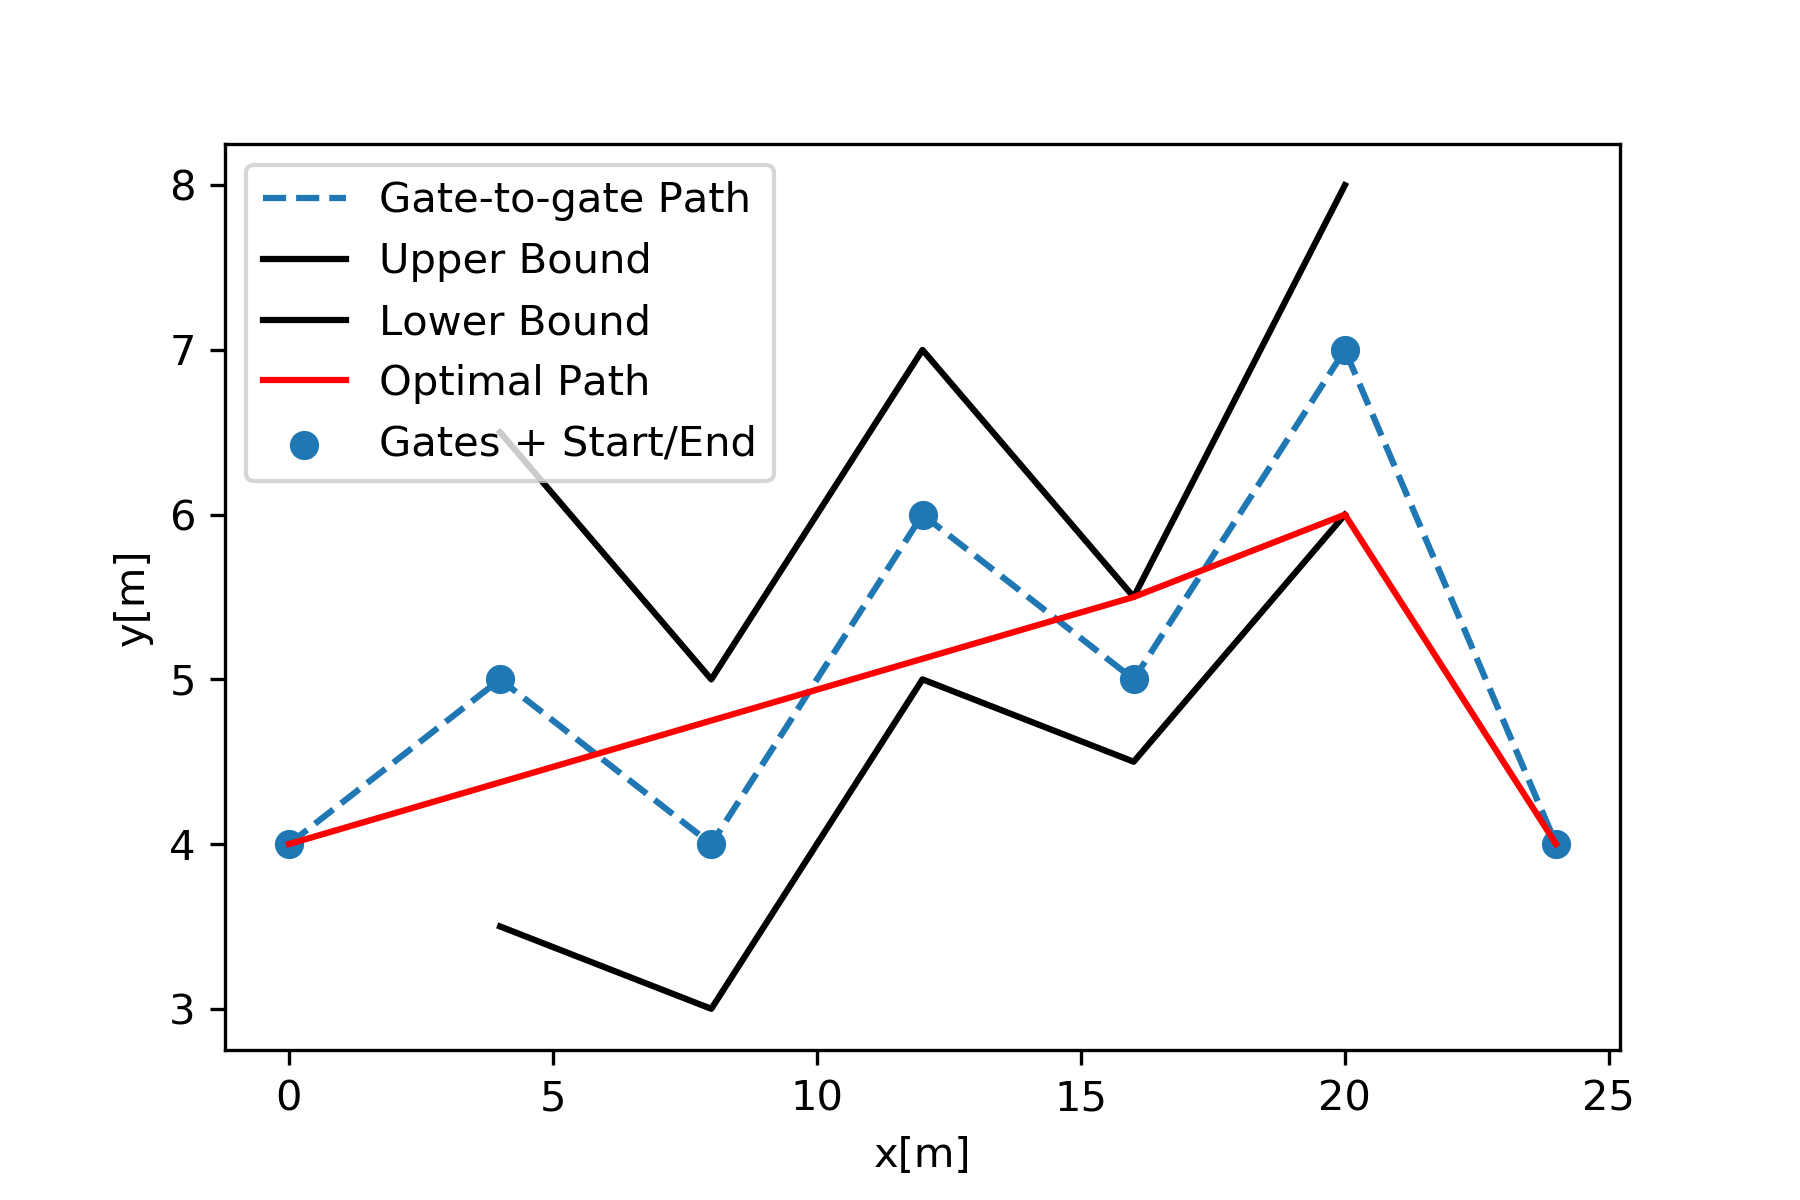
\includegraphics[width=0.5\textwidth]{problem5_sol.png}}
    \end{figure}
  \end{enumerate}
\end{solution}

\end{document}
